\chapter{The Search for Regions of High Charge Trapping}\label{chap:trapping}

LEGEND-200 currently operates detectors up to three times more massive than its predecessors and current R\&D efforts are pushing even beyond this. It was hypothesized that in such large volume detectors, deep hole trapping in the bulk could lead to the severe energy degradation of signals. Given that excellent energy resolution was demonstrated for all the ICPCs in LEGEND, severe charge trapping would have to limited to very small regions far away from the point-contact. However, at the tonne-scale even small underperforming volumes could populate the signal window with energy degraded signals.

Thus far the analysis of Compton data has focused on the creation of a pulse shape library. However, the number -- and not just the pulse shape -- of reconstructed events per voxel can provide valuable information. The superpulse of a given voxel was constructed from a pool of individual events which satisfied two conditions: the sum of energies registered by the ICPC and camera fall within the contained event window (Eq.~\ref{eq:contained_cut}) and the path between the voxel and the camera are physically allowed by the relation of energies (Eq.~\ref{eq:ztheta_IC}). If the energy of a Compton event recorded by the ICPC was sufficiently degraded, it would have fallen out of the energy window and not been reconstructed. Therefore, voxels in regions of the detector which were subject to significant charge trapping are prone to an undercount in the number of reconstructed events. Similarly, voxels outside or in dead regions of the detector should not register any counts. Thus, by comparing the number of counts in a voxel to an expected value, either simulated or measured, regions with significant charge trapping or dead volumes -- at the surface or in the bulk -- may be found. 

\section{Effective Compton Capture Rate}
Given a contained event window, and other set parameters like the rate of the \CsS{} source, the number of reconstructed events per voxel depends on three experimental variables: the position of the camera, denoted by index $i$, and the cleaning cut efficiency, $\varepsilon^{cut}_i$, and the measurement time, $T_i$, at each camera position. To compare across measurements or to simulation, the camera positions must match at every $r$, and the dependency on measurement time and efficiency needs to be removed. The latter is achieved by calculating the effective Compton capture rate, defined as:
\begin{equation}
	\mathcal{R}^c(r,z) = \sum_{i = 1}^{N_\text{cam}}\left(\frac{1}{\varepsilon^{cut}_iT_i}\int_{z-\Delta z}^{z+\Delta z}f_i(z_\theta)dz_\theta\right)
	\label{eq:effectve_compton_capture_rate}
\end{equation}
where $N_\text{cam}$ is the number of camera positions at given $r$, $f(z_\theta)$ is the $z$-distribution of reconstructed events and $\varepsilon^{cut} = \varepsilon^{hp}\varepsilon^{burst}\varepsilon^{so}\varepsilon^{ln}$ are the hard pileup, burst, slope offset, and LN$_2$ cut survivals. Note that the subindexes have been dropped for clarity. Unlike the others, the distribution of hard pileup is not uniform in energy. Therefore, the hard pileup cut efficiency is evaluated within the contained event window. The other efficiencies are calculated using the entire spectrum for increased statistics. Examples of $f(z_\theta)$ (and their direct sum) are shown in Fig.~\ref{fig:z_reconstruction_combined}. The effective Compton capture rate can be thought of as the rate of Compton events captured by the large camera at a single position, whose sometimes overlapping pixel positions, match those of all the camera positions combined. This quantity is shown for 1- and 2-hit events for data taken at 3500\,V and 3100\,V bias in Fig.~\ref{fig:capture_rate}. 
\begin{figure}[htb]
    \centering
    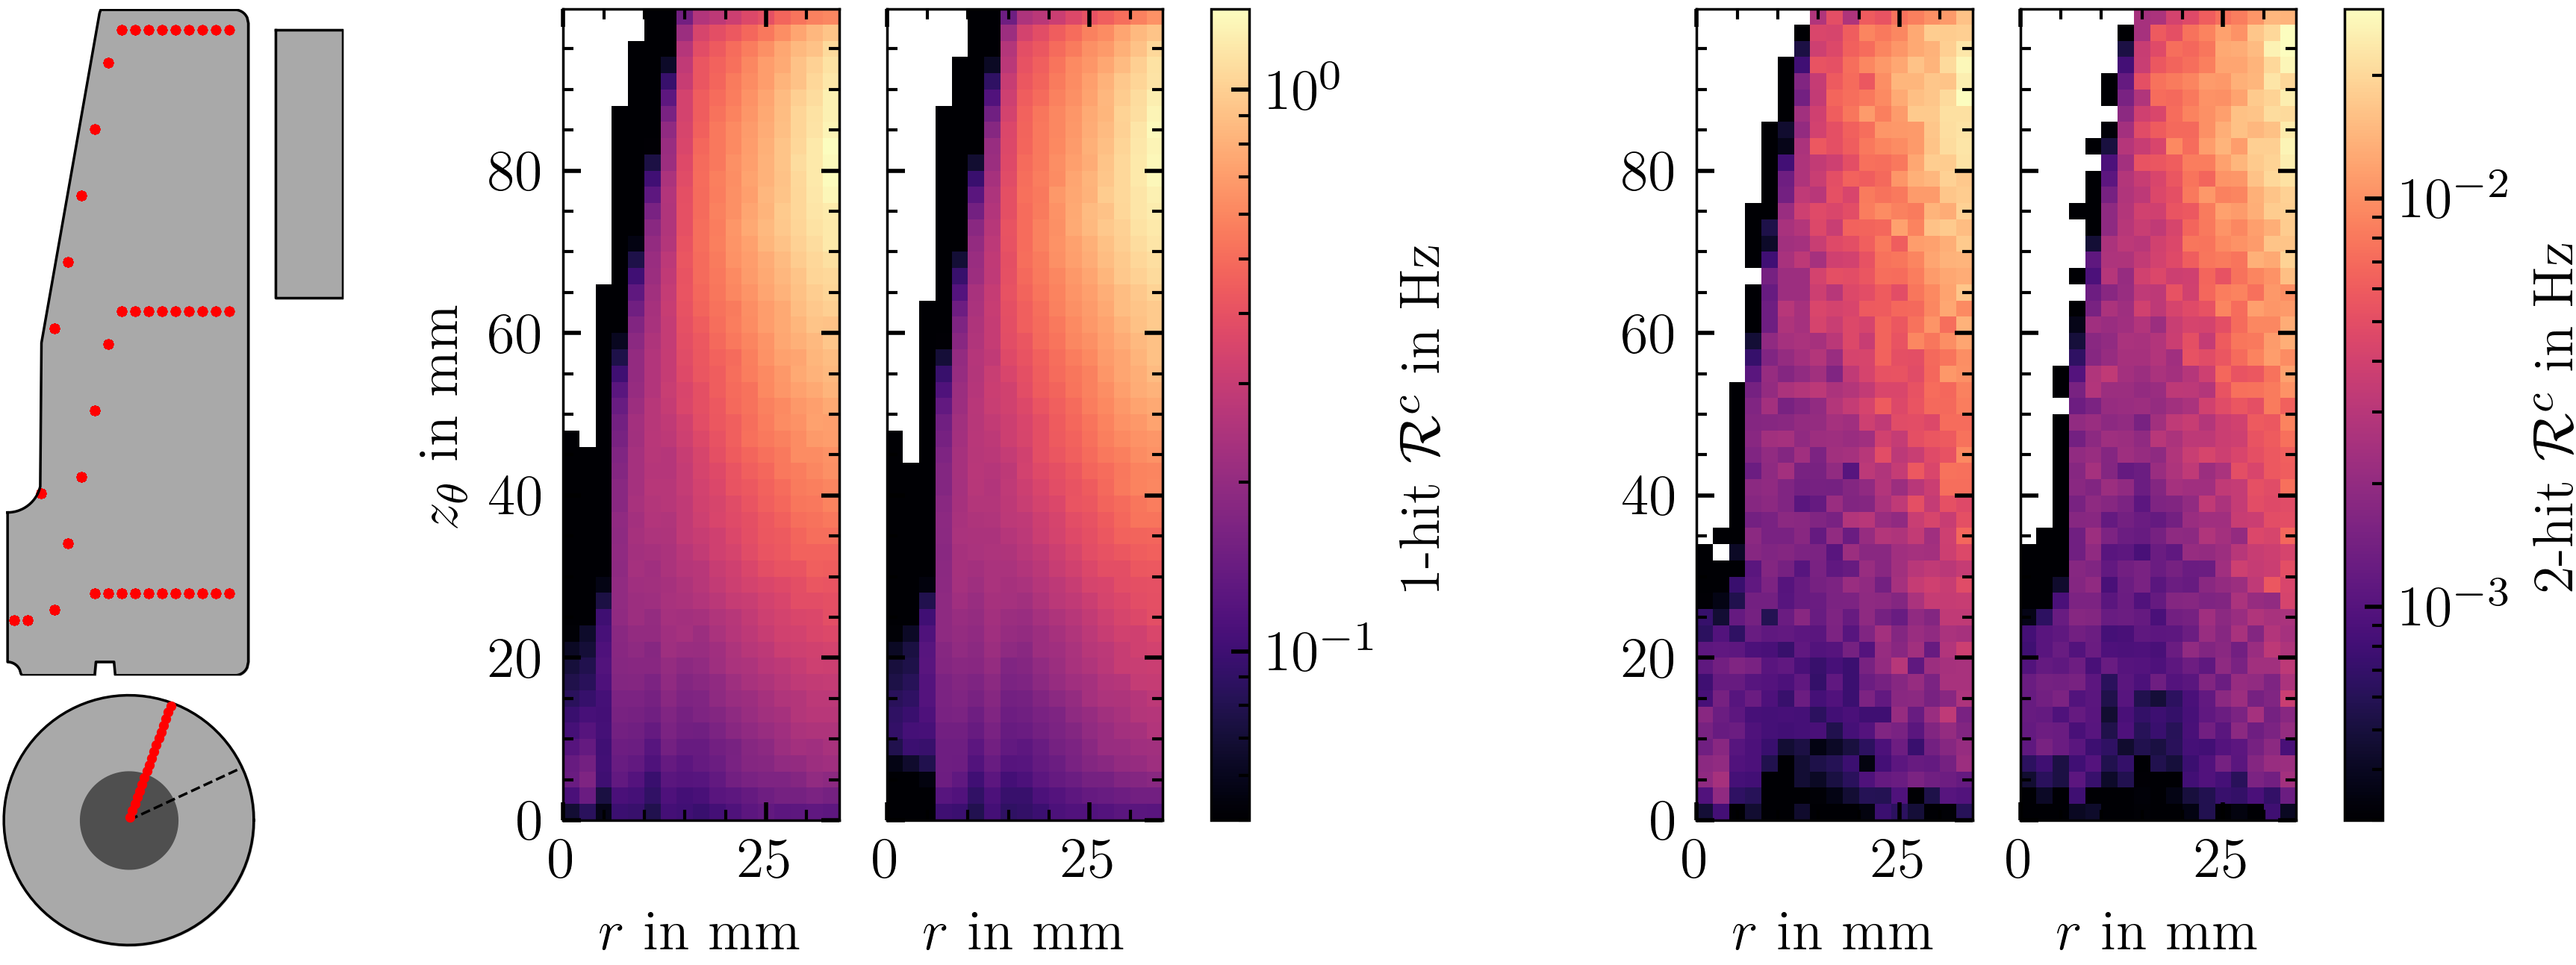
\includegraphics[width=6in]{figs/trapping/biascomp_fast_axis_rates.png}
    \caption{Effective Compton capture rate for (from left to right) 1-hit events with the detector at 3500\,V and 3100\,V bias and 2-hit events with the detector at 3500\,V and 3100\,V bias along the $\left<1\,0\,0\right>$ axis of the detector. The scan at 3100\,V was performed with the same camera positions (shown in the pictogram) as the 3500\,V scan.}
	\label{fig:capture_rate}
\end{figure}

There are visible fluctuations in rate between radii, in particular for $r < 15$\,mm. This is evident in the 1-hit heat maps as brighter color lines. For such radii, there is a particularly large overlap of camera positions. These fluctuations and the observed exponential decay in rate along the $z$-axis can be corrected for by dividing the rate by a simulated efficiency which accounts for the geometry of the system and gamma attenuation. 

\section{Compton Scatter Collection Efficiency}

A full Monte Carlo simulation, which accounts for all the interactions in the source collimator, detector, camera and surrounding materials is required to calculate the expected 1- and 2-hit event $\mathcal{R}^c$. However, the exact ratio of measured to expected $\mathcal{R}^c$ is not needed to find regions with rate underfluctions. Rather, the measured $\mathcal{R}^c$ of a voxel can be compared to those surrounding it. Nevertheless, two predominant physical effects must be corrected for before a fair comparison can be made: gamma attenuation and geometrical efficiency. Both of these effects are accounted for in the \textit{simulated} Compton scatter collection efficiency, $\varepsilon^c$, which is calculated for a voxel centered at $(r,z)$ and camera position $i$ as follows:
\begin{itemize}
	\item The survival fraction of gammas is calculated as $e^{-\mu(E_\text{in})(z^\text{top}(r) - z)}$ where $\mu(E_\text{in})$ is the total linear attenuation coefficient of $E_\text{in}=662$\,keV gammas, and $z^\text{top}(r)$ describes the geometry of the top of the detector at a given $r$. The incoming gamma survival probability is shown in the leftmost heatmap in Fig.~\ref{fig:acceptance_corr}. 
	\item A gamma ray is traced from origin $(r,z)$ and direction given by $(\theta^\prime, \phi^\prime)$ in spherical coordinates. In this coordinate system, $\theta^\prime = \theta - 90^\circ$, where $\theta$ is the Compton scattering angle.  The distance of Ge trasversed by the gamma ray, $l_\gamma(r,z,\theta^\prime, \phi^\prime)$, is calculated according to the geometry of the detector. Thus, the probability of the gamma escaping the detector is given by $e^{-\mu(E_\gamma)l_\gamma(r,z,\theta^\prime,\phi^\prime)}$, where $\mu(E_\gamma)$ is the total linear attenuation coefficient of gammas with $E_\gamma = E_\text{out}(\theta)$ given by Eq.~\ref{eq:compton_intro}.
	\item $N_\gamma$ gamma rays are traced from the $(r,z)$. The simulated $\theta$ follow the distribution given by the Klen-Nishina formula (Eq.~\ref{eq:klein-nishina}), while the simulated $\phi^\prime$ follow a uniform distribution. The gamma escape probabilities are summed over for gammas rays which intersect the camera plane -- simulated as a single rectangular plane bisecting the true camera (see leftmost panel of Fig.~\ref{fig:acceptance_corr}) -- and divided by $N_\gamma$. The outgoing gamma survival and collection probability is shown in the middle heatmap in Fig.~\ref{fig:acceptance_corr}. 
\end{itemize}
\begin{figure}[htb]
    \centering
    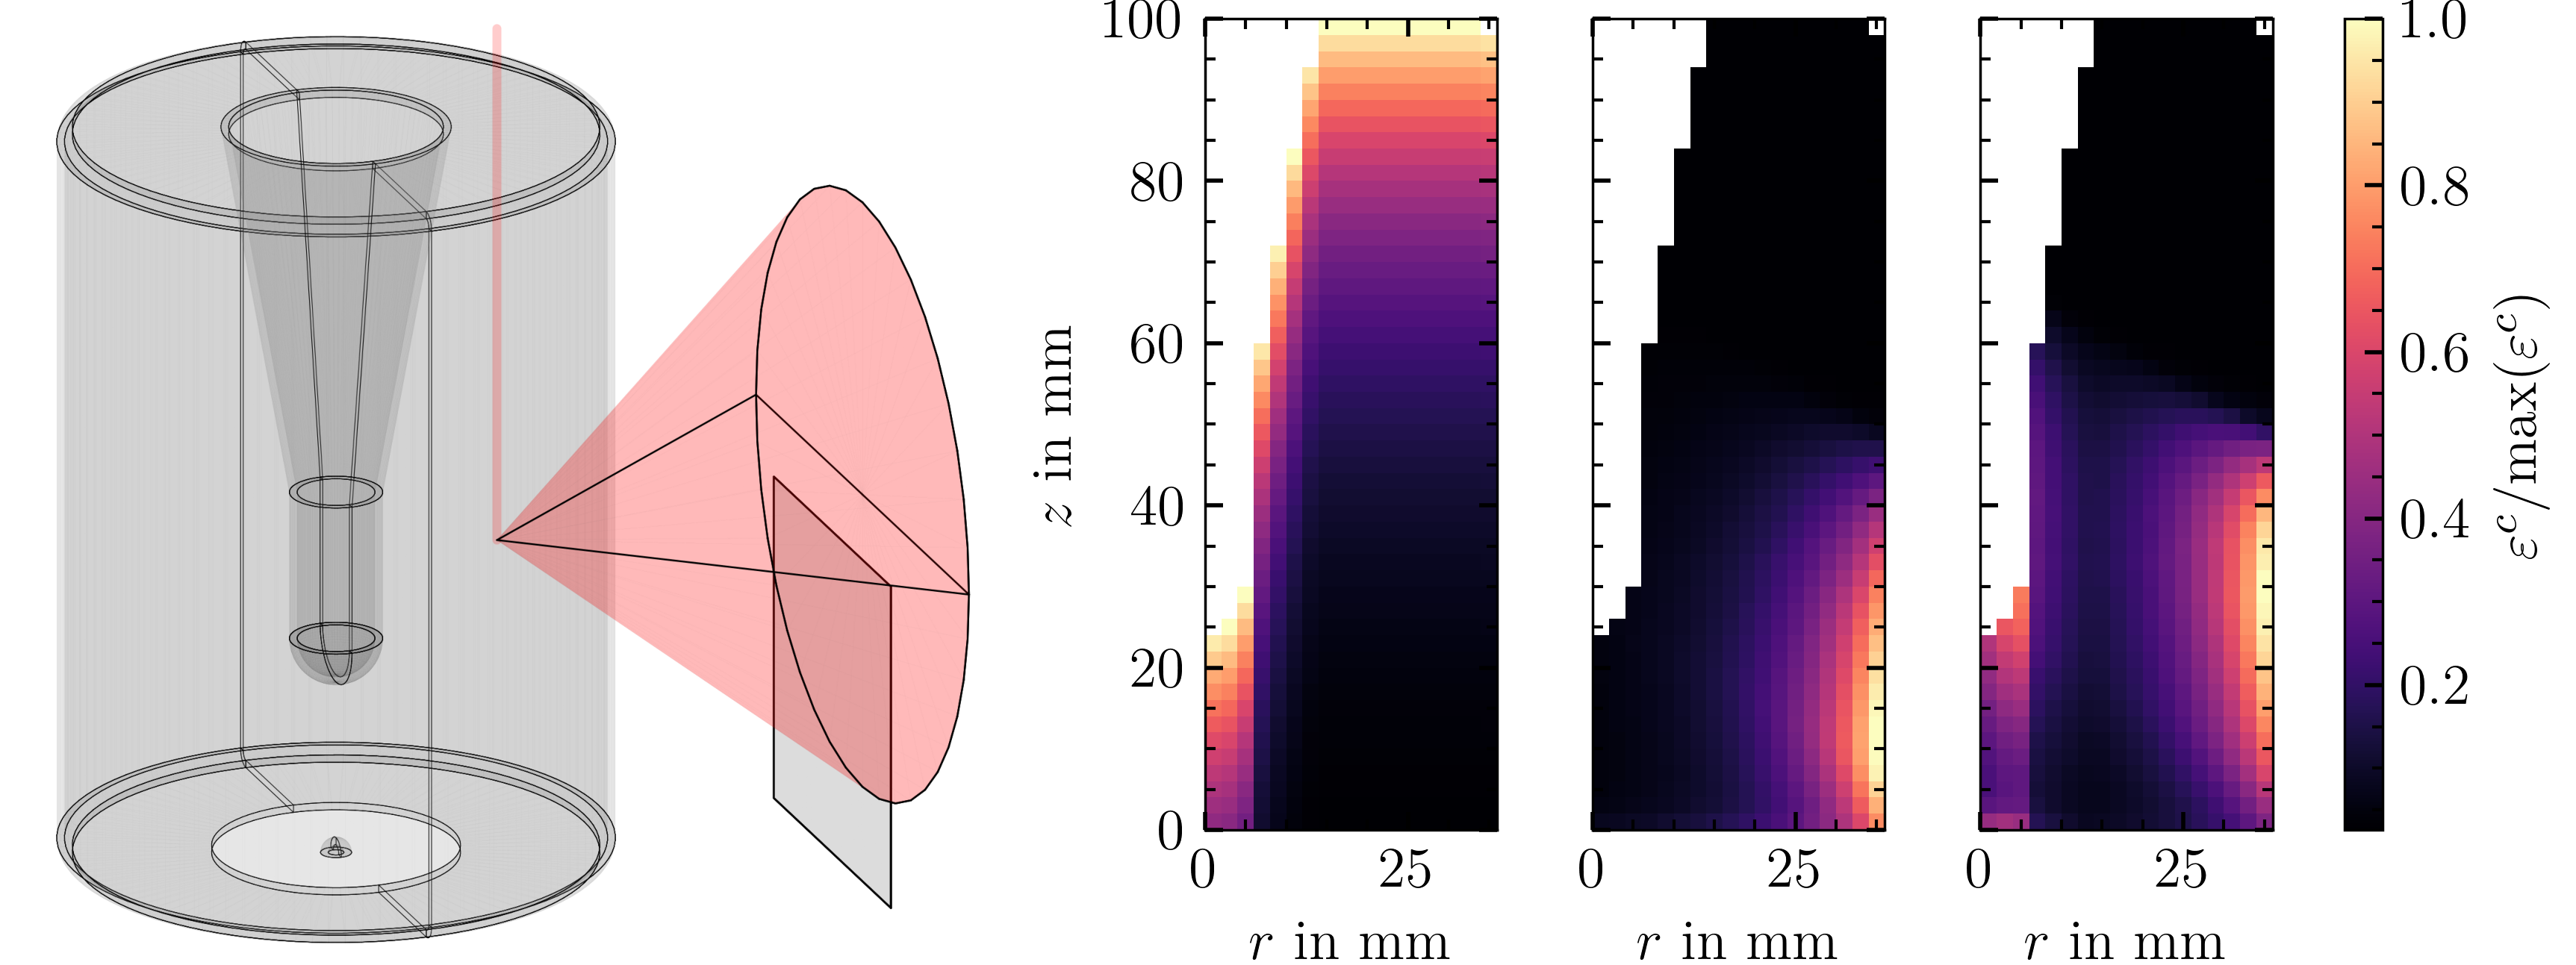
\includegraphics[width=6in]{figs/trapping/accemptance_corr.png}
    \caption{A visual representation of incoming and outgoing gammas is shown on the left, where the $\theta^\prime$ distribution has been truncated at $\pm30^\circ$. The incoming gamma survival probability and the outgoing gamma survival and collection probability are shown in the leftmost and middle heatmaps respectively. The multiplication and renormalization of these values produces the heatmap on the right.}
	\label{fig:acceptance_corr}
\end{figure}
The incoming gamma survival probability is multiplied by the outgoing gamma survival and collection probability to obtain $\varepsilon^c$ for a single camera position. This quantity is shown in the rightmost heatmap in Fig.~\ref{fig:acceptance_corr}.
Summing the contribution from each camera position gives the full expression for Compton scatter collection efficiency:
\begin{equation}
	\varepsilon^{c}(r,z) = e^{-\mu(E_\text{in})(z^\text{top}(r) - z)}\sum_{i = 1}^{N_\text{cam}}\left(\frac{1}{N_\gamma}\sum_{\gamma\in\text{cam}_i}e^{-\mu(E_\gamma)l_\gamma(r,z,\theta^\prime,\phi^\prime)}\right)
	\label{eq:compton_eff}
\end{equation}

Except for the grove at the bottom, the ICPC, and thus path lengths through it, are simulated true to form. Simulated gammas interact only once in the detector. As previous chapters covered in detail, multiple steps are taken to ensure that reconstructed events only interact once in the detector as well. In the simulation, gammas passing through the plane of the camera are assumed to be collected with 100\% probability. This is far from reality; however, since a simulated rate is not needed, it suffices that the camera collection probability be independent of $\theta^\prime$ and $\phi^\prime$. This is certainly not the case for gammas hitting close to the edges of the camera. However, over most of the camera area the angle dependence can be limited by restricting $\theta$ to $(90\pm30)^\circ$. Note that the Compton reconstruction in data is also most trusted for this range. Additionally, the $\phi^\prime$ range is limited by geometry to lie well between $-28^\circ$ and $45^\circ$. Secondary effects such as this angle dependency may be added to the model as needed in future studies. Note that the simulation can be run in under a minute for the entire radial slice. This poses a considerable advantage over a full Monte Carlo, allowing for multiple camera configurations to be tested during the design stages of the experiment. 

\section{Efficiency Corrected Effective Compton Capture Rate}

The simulated Compton scatter collection efficiency models the relation of effective Compton capture rates amongst voxels very well. This can be seen in Fig.~\ref{fig:rate_vs_acceptance}, where the normalized $\mathcal{R}^c$ is shown for 1- and 2-hit events on the left and the simulated normalized $\varepsilon^{c}$ on the right. The normalization provides the means of comparing the rate to the efficiency. For clarity, only one camera position (at given $r$) is used in this example. An energy cut is applied in data such that $\theta$ is restricted to $(90\pm30)^\circ$ as in simulation. Recall that the validation used for 2-hit events removes detector multi-site events by construction. In this case the $AvsE$ cut is applied to remove the small contamination of multi-site events that the validation misses. The $AvsE$ cut is also applied to 1-hit events. In this case, however, it is the only line of defense against multi-site and other misreconstructed events.
\begin{figure}[htb]
    \centering
    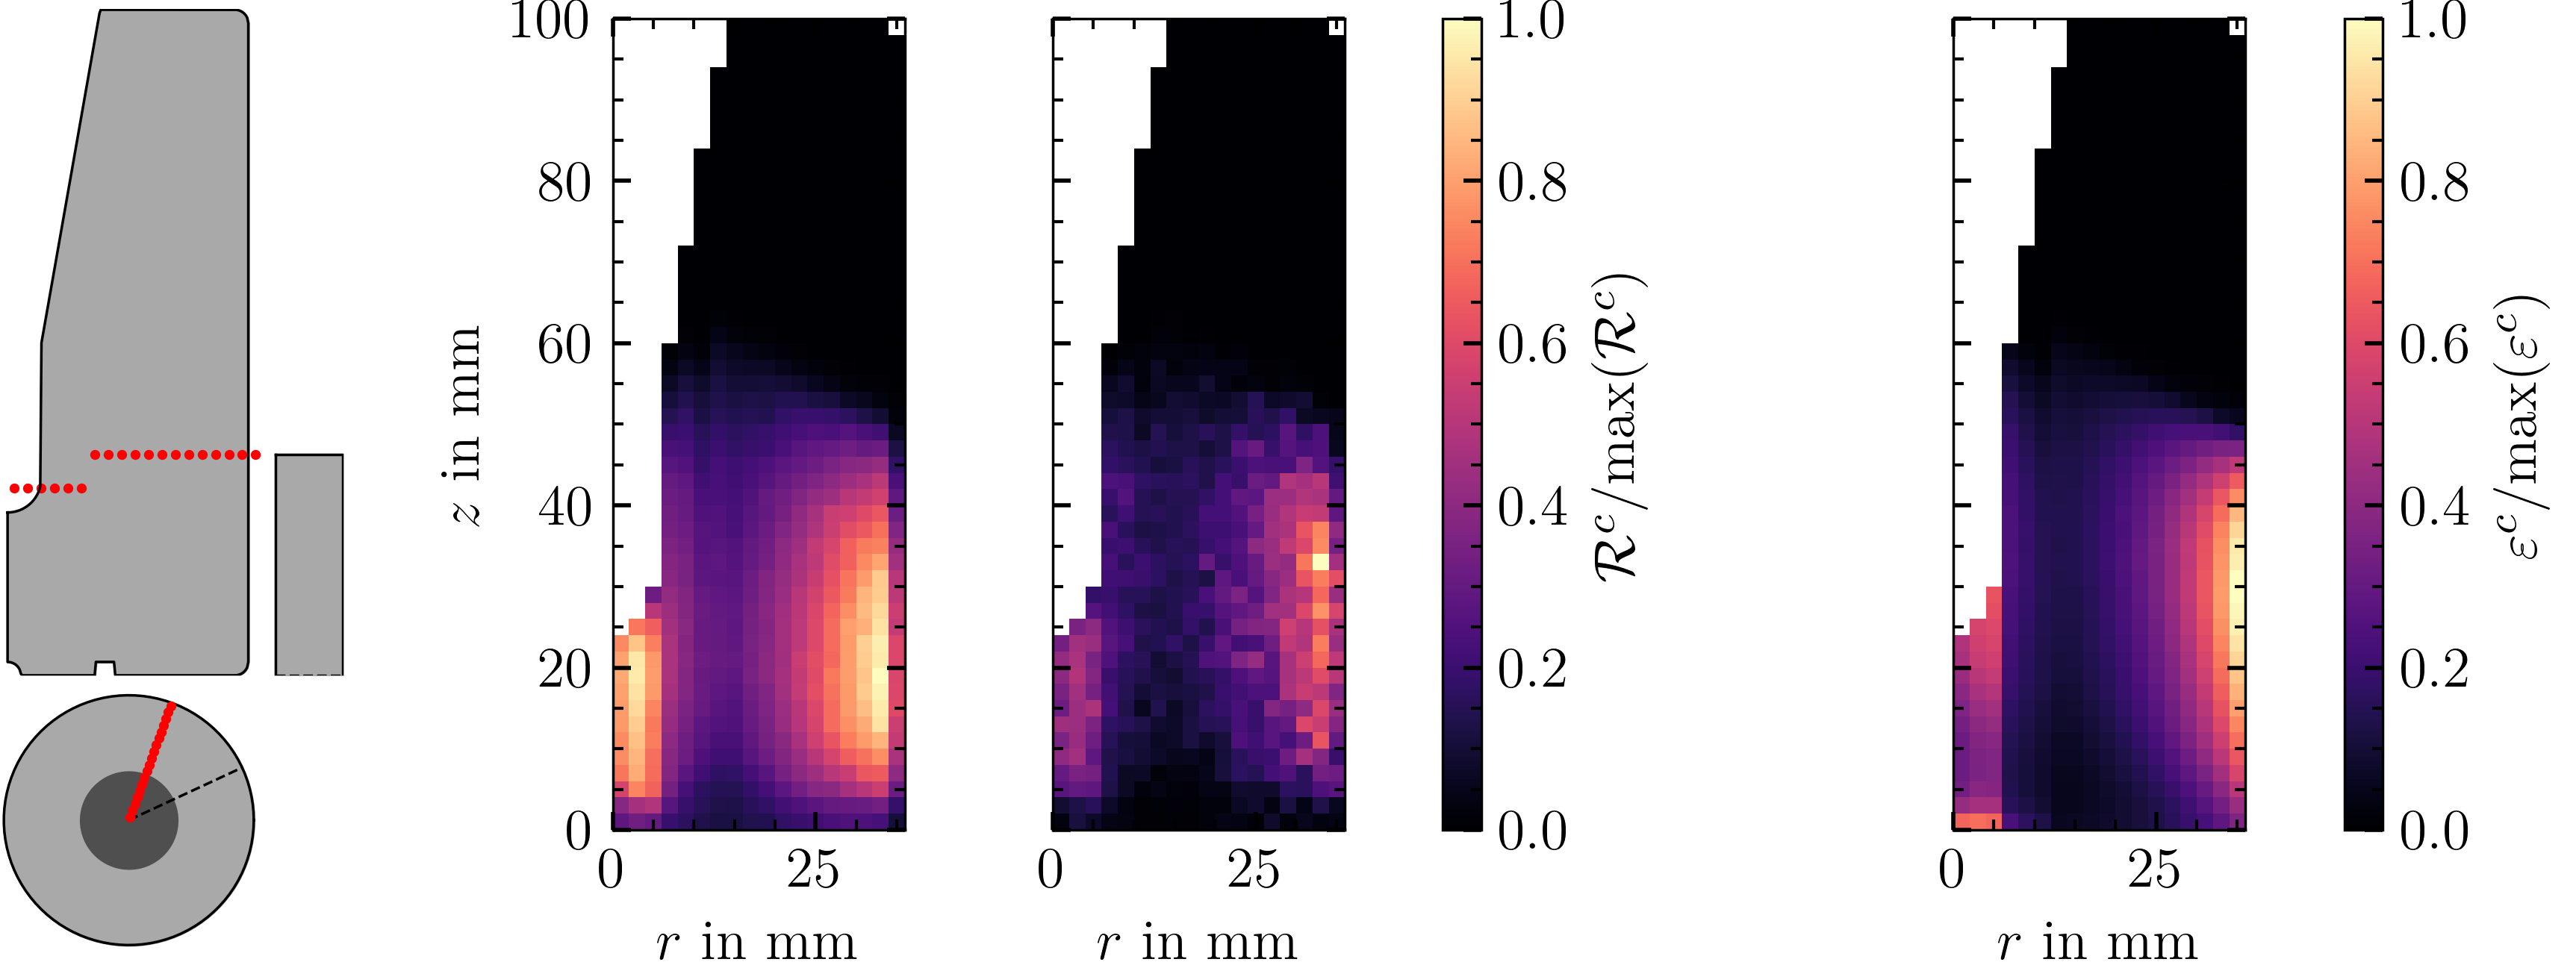
\includegraphics[width=6in]{figs/trapping/rate_vs_acceptance.png}
    \caption{From left to right: 1- and 2-hit $\mathcal{R}^c$ and $\varepsilon^{c}$ for the camera position at given $r$ -- along the $\left<1\,0\,0\right>$ axis of the detector -- shown by the pictogram.}
	\label{fig:rate_vs_acceptance}
\end{figure}

An excess can be seen in the normalized 1-hit $\mathcal{R}^c$ in the lower central region of the detector arm with respect to the normalized $\varepsilon^c$. This is exactly where most misreconstructed events are expected. Nevertheless, the normalized 2-hit $\mathcal{R}^c$ matches the simulation very well. 

Now including all camera positions, a comparison can be made for the full detector. By dividing the normalized $\mathcal{R}^c$ by the normalized $\varepsilon^c$ underfluctuations in event rate can be found. The efficiency corrected effective Compton capture rate, $(\mathcal{R}^c/\text{max}(\mathcal{R}^c))/(\varepsilon^c/\text{max}(\varepsilon^c))$, is shown in Fig.~\ref{fig:acceptance_corr_rate} for data taken at 3500\,V and 3100\,V. The color scale is centered at one, such that underfluctuations appear in blue and overfluctuations in red.
\begin{figure}[htb]
    \centering
    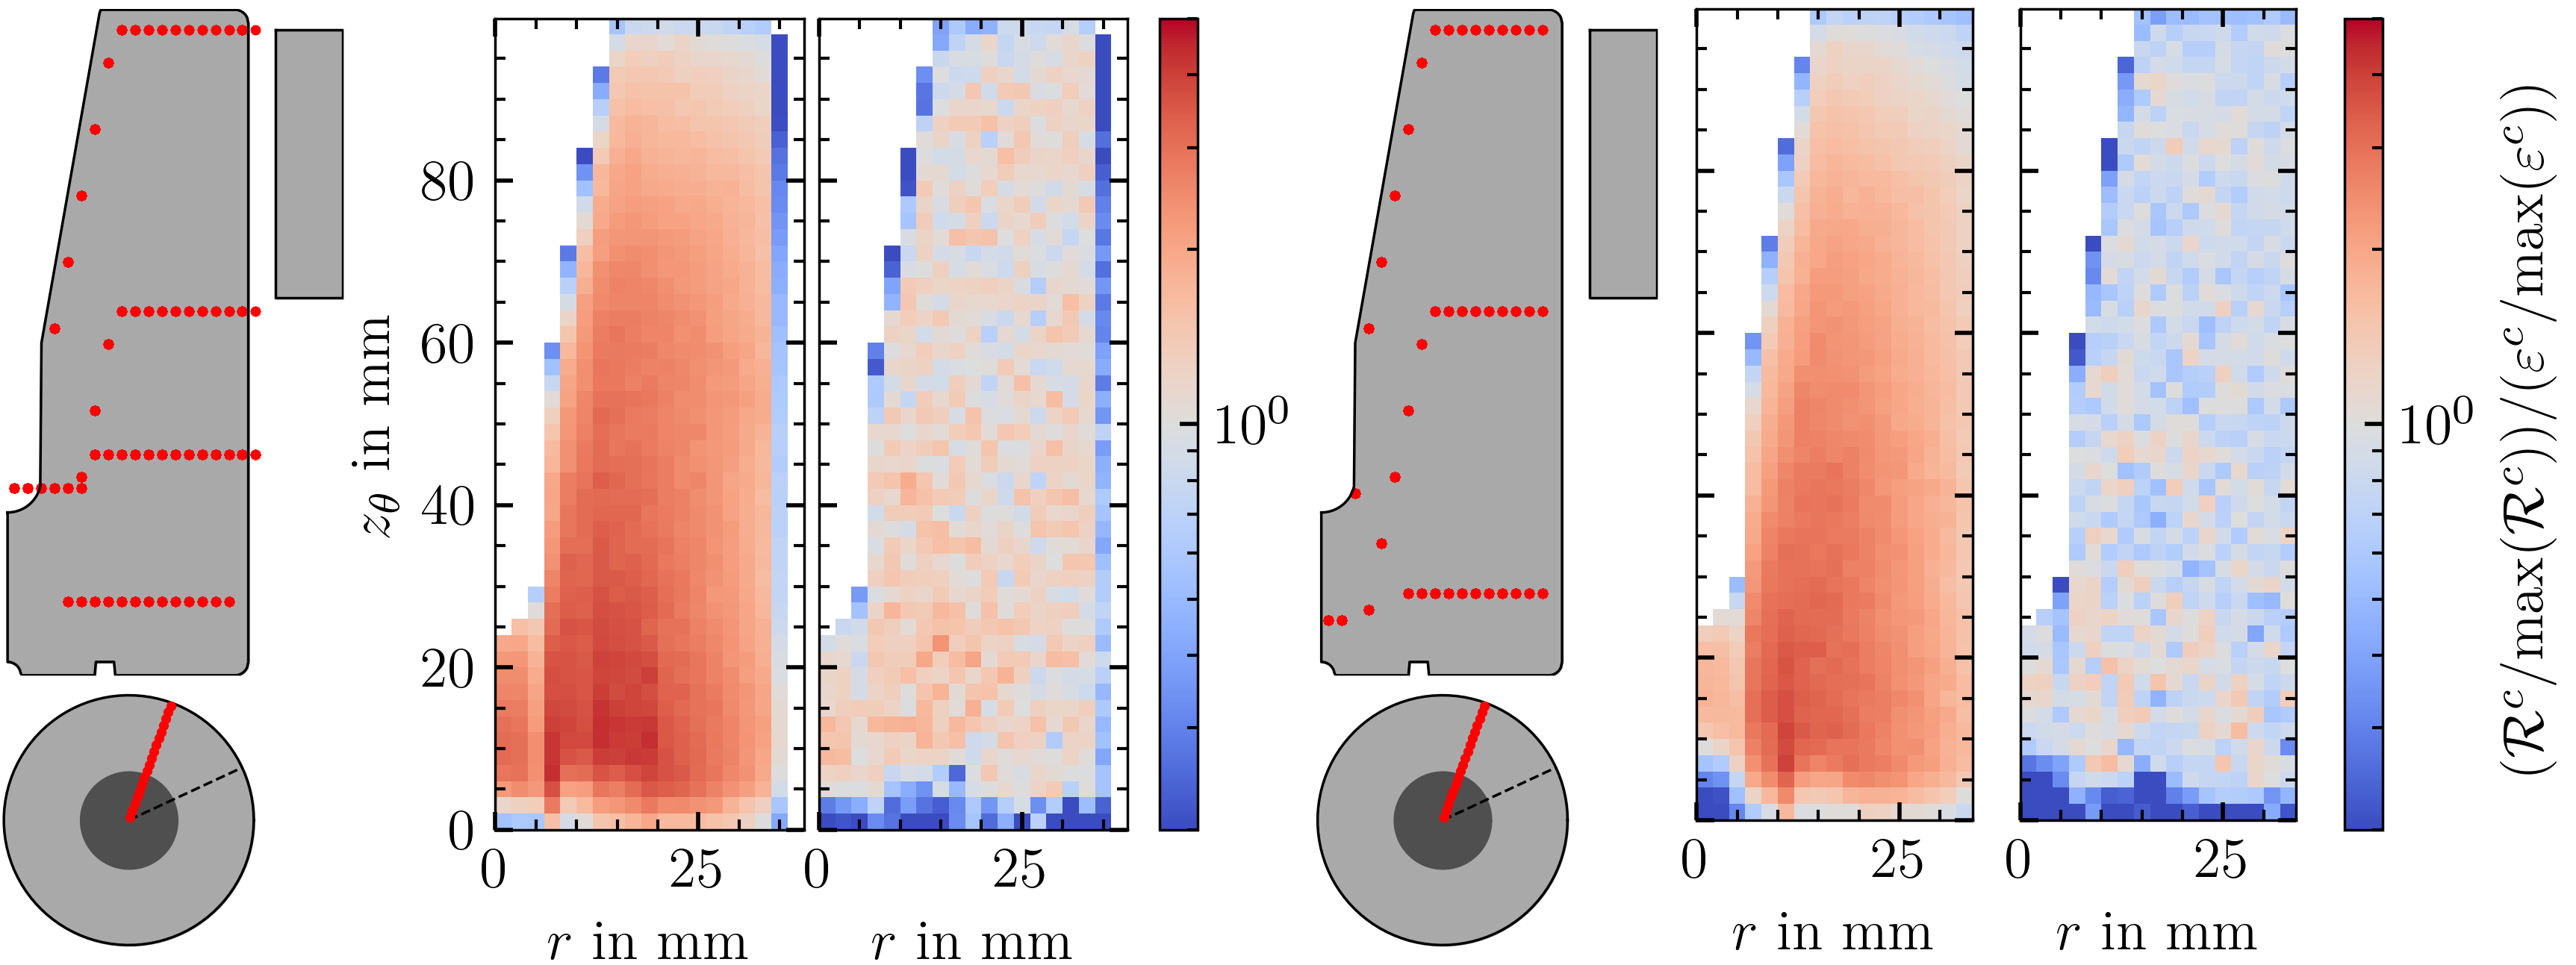
\includegraphics[width=6in]{figs/trapping/acceptance_corr_rate.png}
    \caption{1- and 2-hit event efficiency corrected effective Compton capture rate with the detector at 3500\,V (left two panels) and 3100\,V bias (right two panels) along the $\left<1\,0\,0\right>$ axis of the detector. The logarithmic color scale is centered a one, with extremes at 1/5 and 5.}
	\label{fig:acceptance_corr_rate}
\end{figure}

For 1-hit heatmaps there is a strong contamination of misreconstructed events, seen as a red area spanning most of the detector and concentrated at the bottom. However, for 2-hit events the bulk is mostly featureless, with a slight average bulk overfluctuation at 3500\,V and underfluctuation at 3100\,V. The lack of features throughout the bulk constitutes evidence that significant charge trapping does not take place. It is concluded that at 95\,K the energy recorded by the detector falls within the confines of the established energy resolution models for gammas impinging throughout the bulk.

Common to all heatmaps, consistent underfluctuations are seen at detector edges. These regions are 1-voxel thick, consistent with the 1\,mm n$^+$ dead layer assumption. If the n$^+$ layer is in fact being imaged, a difference in corrected rate should be seen at the bottom of the detector at $r=16$\,mm, where this layer ends. Nevertheless, this feature is too small to be imaged, particularly in an area with very low statistics. Note that the 3100\,V scan did not go all the way to the outer edge of the detector and hence no under fluctuation is seen at the edge of the heatmap. However, a larger feature is consistently imaged at both biases. Since the detector groove -- located at ($r = [13,16]$, $z = [0,2]$)\,mm -- is not included in the simulation, a strong underfluctuation is expected. This is seen in data. 

Finally, a surprising feature was found at 3100\,V. A significant underfluctuation 3-4 voxels in radius is found at the point contact. Although the detector was determined to be depleted at 2950\,V while biasing, this feature is consistent with the shape of an undepleted region when approaching full bias voltage. An analysis of pulse shapes in a HV scan starting at 3500\,V and going down in steps of 100\,V, determined that the bias voltage had in fact shifted to around 3350\,V, confirming the undepleted hypothesis. Such shifts in bias voltage are possible, given that as the detector settles there is a thermal release of impurities from deep hole traps. This release increases the net impurity concentration, thus increasing the bias voltage asymptotically over time.


\section{Effective Compton Capture Rate Ratios}

Since the 2-hit efficiency corrected effective Compton capture rate is featureless at 3500\,V, these data can be used to search for underfluctuations in rate at other biases. In this manner, a direct data-based rate-to-rate ratio can be computed, as opposed to the simulation-based double ratios used in the last section. A direct ratio of rates poses a considerable advantage, allowing for the use of high statistics 1-hit data as well. Although 1-hit data contains a considerable contamination of misreconstructed events (as seen in Fig.~\ref{fig:acceptance_corr_rate}) the contamination -- mostly from multi-site events -- at a given voxel is expected to remain fairly constant at different biases. Thus, underfluctuations in correctly reconstructed events should still be seen. Fig.~\ref{fig:biascomp_axis_ratios} shows the ratio of effective Compton Capture rates at 3500\,V and 3100\,V bias, $\mathcal{R}^c_{3100\,\text{V}}/\mathcal{R}^c_{3500\,\text{V}}$.
\begin{figure}[htb]
    \centering
    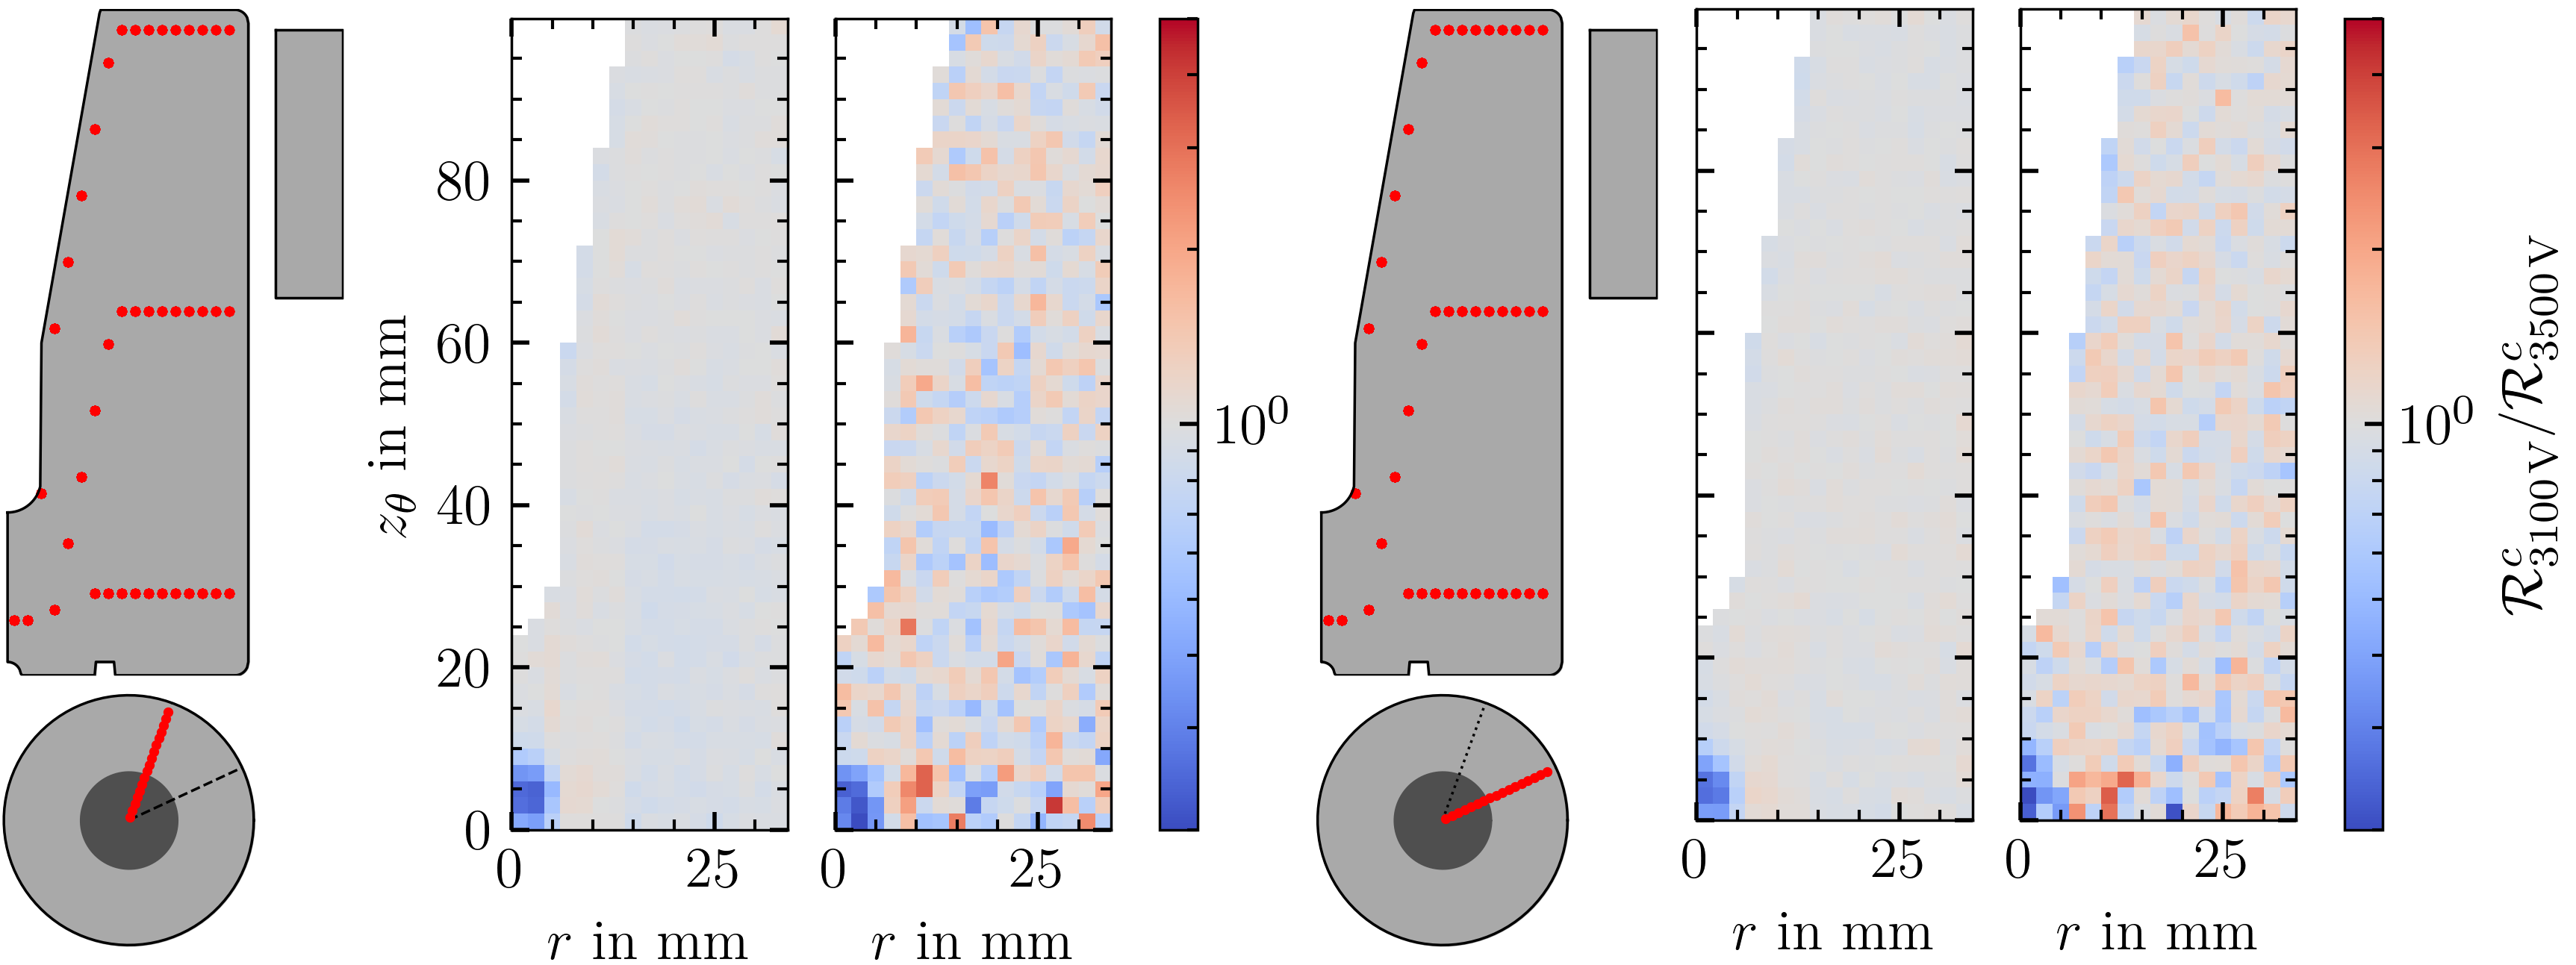
\includegraphics[width=6in]{figs/trapping/biascomp_axis_ratios.png}
    \caption{The ratio of effective Compton Capture rates at 3500\,V and 3100\,V bias is shown for the $\left<1\,0\,0\right>$ and the $\left<1\,1\,0\right>$ axes of the detector on the left and right respectively. For each axis the rate ratio calculated from 1- and 2-hit events is shown on the left and right respectively.}
	\label{fig:biascomp_axis_ratios}
\end{figure}

The depletion surface is clearly present in the 1- and 2-hit event heatmaps. As with the simulation-based double ratios, the rest of the bulk of the 2-hit event heatmap is featureless, however, this is now true for the 1-hit event heatmap as well. The latter supports the hypothesis that the contamination of misreconstructed events at a given voxel remains constant at different biases. An energy cut which restricts the Compton angle, $\theta$, to $(90\pm30)^\circ$ was applied to the data shown. To avoid introducing differences in $AvsE$ cut efficiency at the different biases, this cut was not applied. 

As shown in Fig.~\ref{fig:bubble_3100} -- an enlargement of the leftmost panel of Fig.~\ref{fig:biascomp_axis_ratios} -- the underfluctuation in $\mathcal{R}^c_{3100\,\text{V}}/\mathcal{R}^c_{3500\,\text{V}}$ is statistically significant at the depletion surface for 1-hit events.
\begin{figure}[htb]
    \centering
    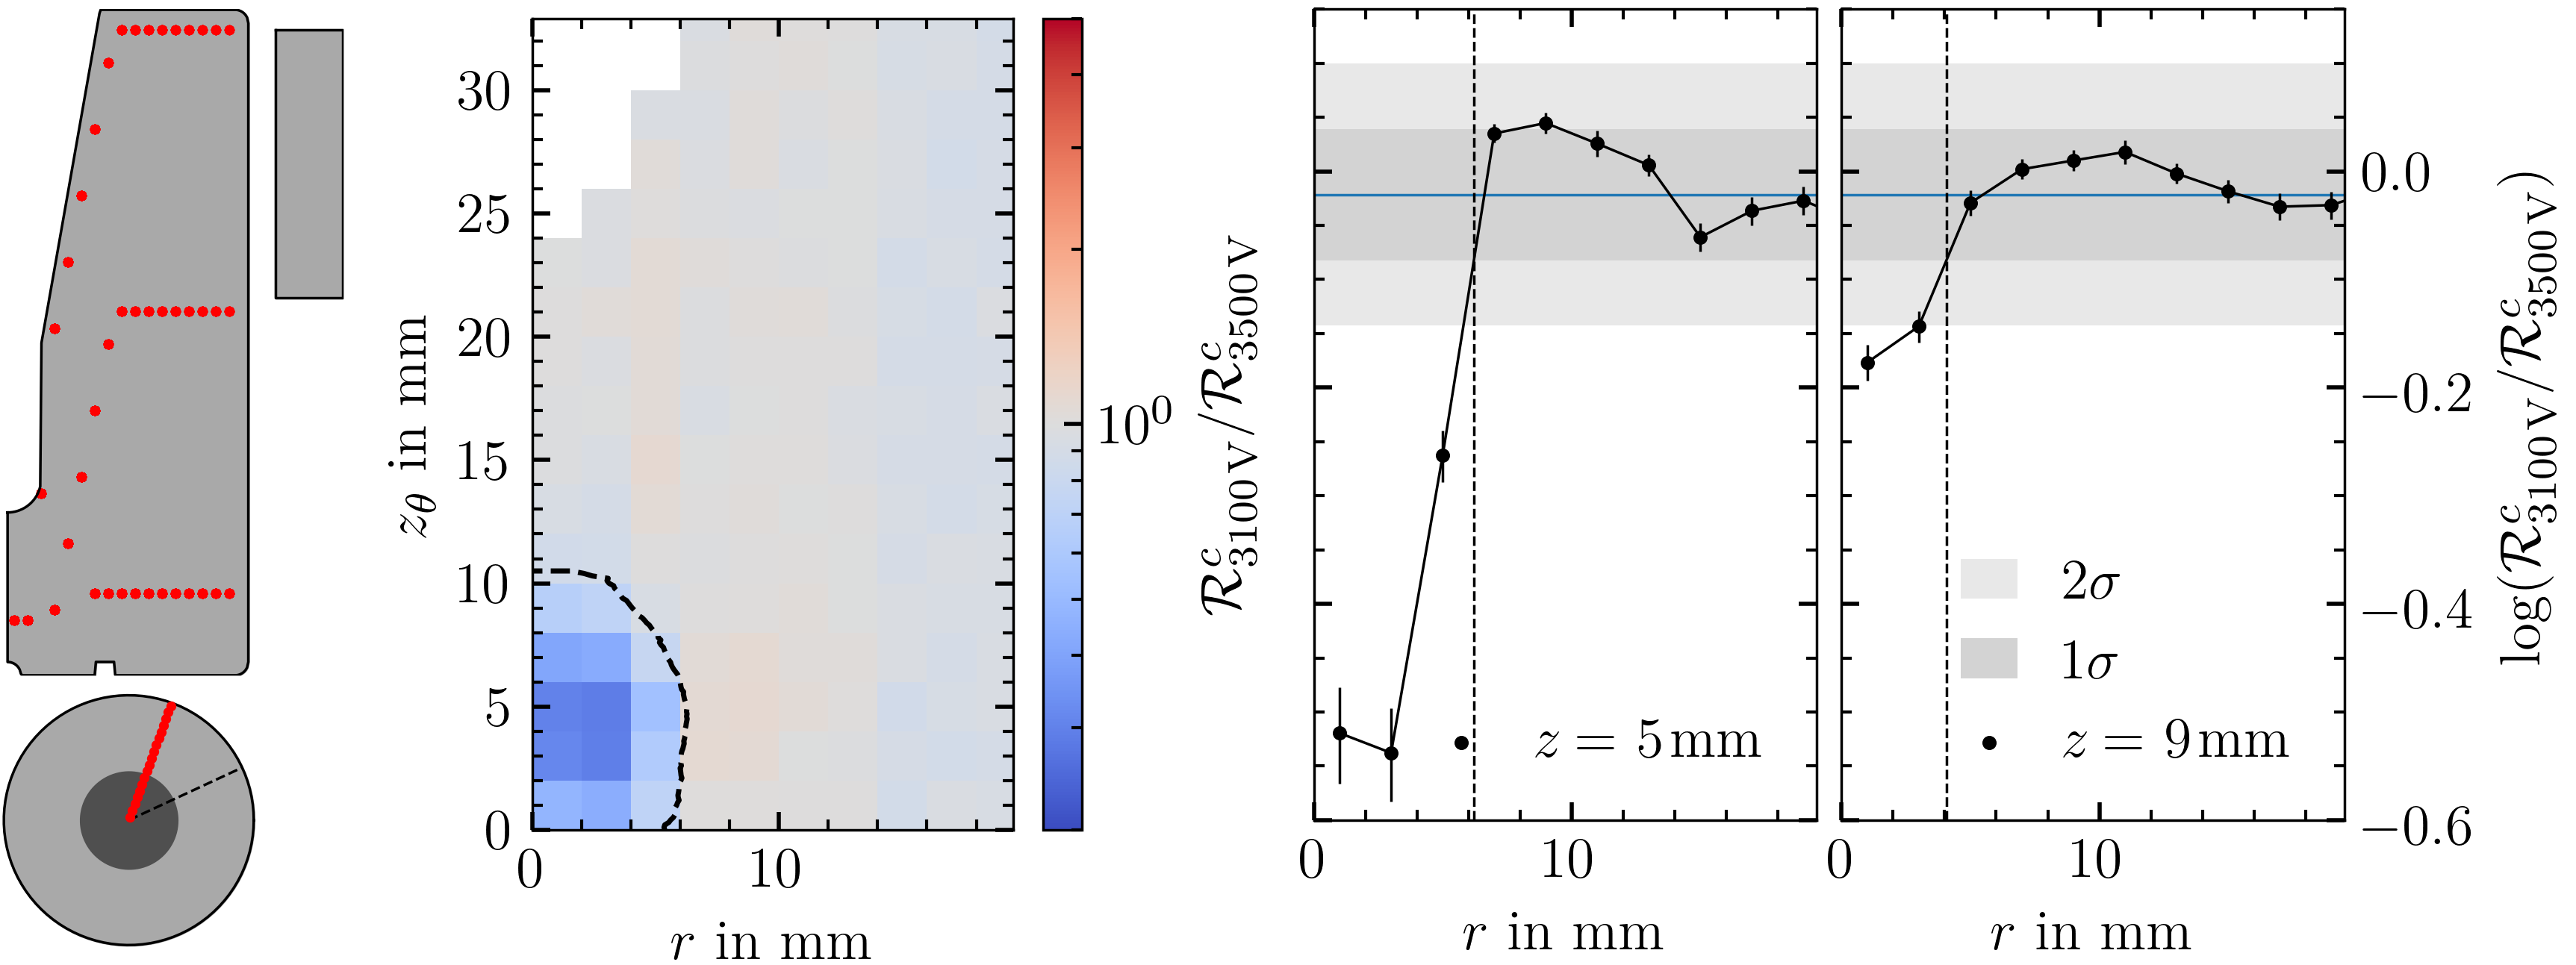
\includegraphics[width=6in]{figs/trapping/biascomp_bubble.png}
    \caption{The ratio of effective Compton Capture rates at 3500\,V and 3100\,V bias is shown for the $\left<1\,0\,0\right>$ for 1-hit events. The statistical analysis described in the text is shown on the two panels on the right for $z=5$\,mm and $z=9$\,mm. The mean $\log(\mathcal{R}^c_{3100\,\text{V}}/\mathcal{R}^c_{3500\,\text{V}})$ is shown as a blue horizontal line.}
	\label{fig:bubble_3100}
\end{figure}
The depletion surface, is calculated as the $r$ at which the interpolated $\log(\mathcal{R}^c_{3100\,\text{V}}/\mathcal{R}^c_{3500\,\text{V}})$ dips under a 1$\sigma$ deviation from the mean. This value is shown as dashed vertical lines in Fig.~\ref{fig:bubble_3100}. This calculation is repeated at all $z$, that is by varying $z$ continuously in Eq.~\ref{eq:effectve_compton_capture_rate} at 3100\,V and 3500\,V, to create the boundary shown in the figure. Using this boundary, and assuming rotational symmetry, the undepleted volume at 3100\,V is 995.5\,mm$^3$. 